% -------------------------------- SVILUPPO -------------------------------------

\chapter{Probabilità}
\section{Spazi di probabilità}
\subsection{Probabilità uniforme}
\begin{itemize}
	\item P(A) = $\dfrac{|A|}{|\Omega|}$ = $\dfrac{Casi \ possibili}{Casi\  totali}$
\end{itemize}
\subsection{Probabilità condizionale}
\begin{itemize}
	\item $P(A \cap B) = P(A|B) \cdot P(B)$ (dipendenza)
	\item $P(A \cap B) = P(A) \cdot P(B)$  (indipendenza)
	\item $P(B|A) = \dfrac{P(A|B) \cdot P(B)}{P(A)}$
	\item $P(A|B) = P(A) = \dfrac{P(A \cap B)}{P(B)}$ (valido se c'è indipendenza)
\end{itemize}
\subsection{Formula di bayes}
\begin{itemize}
	\item $P(B|A) = \dfrac{P(A|B) \cdot P(B)}{P(A)}$
\end{itemize}
\subsection{Probabilità totali}
\begin{figure}[H]
	\centering{}
	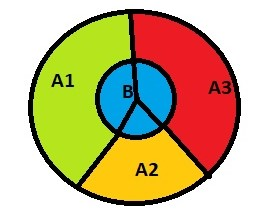
\includegraphics[width=\textwidth]{img/probtotali}
	\label{img:probtotali}
\end{figure}
	$P(B) = P(B \cap A_1) + P(B \cap A_2) + P(B \cap A_3)$ \\ \\
	= $P(A_1) \cdot P(B|A_1) + P(A_2) \cdot P(B|A_2) + P(A_3) \cdot P(B|A_3)$
\newpage
\section{Variabili aleatorie discrete}
\subsection{Densità discreta astratta}
Una funzione $p : \mathbb{R} \rightarrow \mathbb{R}$ \\
è una densità discreta astratta se e solo se: \\
\begin{itemize}
	\item $p(h) \neq 0$;
	\item $p(h) \geqslant 0 \ \ \forall \ \ h \in \mathbb{R}$;
	\item $\displaystyle \sum_{h \in \mathbb{R}} p(h) $ = 1;
\end{itemize}

\subsection{Distribuzioni discrete}
\textbf{Densità uniforme ($d_{x}(k)$)} \\ \\
$
\begin{cases}
	\dfrac{1}{n}\qquad  k = 1 \\  
	0\qquad			 altrimenti \\
\end{cases}
$	\\ \\ \\
\textbf{Densità di Bernoulli( $p_{x}(k)$ )} \\ \\
$
\begin{cases}
	P(A)\qquad\quad  	k = 1 \\  
	1 - P(A)\quad	k = 0 \\
	0\qquad\qquad\quad		altrimenti
\end{cases} \\
$ \\ 

\textbf{Densità binomiale ($p_{x}(k))$} \\ \\
$
\begin{cases}
	p^{k} \cdot(1-p)^{n - k} \cdot \binom{n}{k}\quad  k = 0,...,n \\  
	0\qquad\qquad\qquad\qquad\quad		 altrimenti \\
\end{cases}
$ \\ \\		

\textbf{Densità ipergeometrica (si considera a = successo)} \\ \\
$
\begin{cases}
	\dfrac{\binom{a}{k} \cdot \binom{b}{n - k}}{ \binom{a + b}{n}}\qquad  k = max(n - b), ..., min(n, b) \\  
	0\qquad\qquad\qquad			 altrimenti \\
\end{cases}
$ \\ \\	

\textbf{Densità geometrica modificata (cons. una sequenza con k - 1 insuccessi + 1 successo)} \\ \\
$
\begin{cases}
	(1 - p)^{k - 1} \cdot p\qquad  k = 1,2,3,... \\  
	0\qquad\qquad\qquad\quad			 altrimenti \\
\end{cases}
$ \\ \\	

\textbf{Densità geometrica standard (cons. una sequenza con k insuccessi prima di arrivare al successo)} \\ \\
$
\begin{cases}
	(1 - p)^{k} \cdot p\qquad  k = 1,2,3,... \\  
	0\qquad\qquad\qquad			 altrimenti \\
\end{cases}
$ \\ \\	

\textbf{Densità di Poisson} \\ \\
$
\begin{cases}
	e^{-\phi} \cdot \dfrac{\phi^{k}}{k!}\quad k = 1,2,3,.. \\
	0\qquad\quad\quad			 altrimenti \\
\end{cases}
$ \\ \\	

\section{Variabili discrete multidimensionali}